% Chapter Template

\chapter{Methods: High-Density Model Reduction} % Main chapter title

\label{ch:methods hdmr} % Change X to a consecutive number; for referencing this chapter elsewhere, use \ref{ChapterX}

\lhead{Chapter 4. \emph{Methods: High Density Model Reduction}} % Change X to a consecutive number; this is for the header on each page - perhaps a shortened title

%----------------------------------------------------------------------------------------
%	SECTION: INTRO
%----------------------------------------------------------------------------------------

\section{Introduction}
TODO



\section{High-Dimension Model Representation (HDMR)}
While using SCgPC is one method for creating a reduced-order model for a simulation code $u(Y)$, another
useful model reduction is HDMR\cite{hdmr}, sometimes known as Sobol decomposition because the expansion is
conducive to easily determining Sobol sensitivity coefficients.  HDMR is an ANalysis Of VAriance (ANOVA)
method.

In general, the HDMR expansion involves the sum of several terms, each of which only depends on a subset of
the full input space.  The subsets are developed by integrating out the undesired dimensions.  Letting $H(Y)$
represent the untruncated HDMR expansion of $u(Y)$,
\begin{equation}\label{eq:anova}
  u(Y) = H(Y) = h_0 + \sum_{n=1}^N h_n + \sum_{n_1=1}^N \sum_{n_2=1}^{n_1-1} h_{n_1,n_2} + \cdots +
  h_{1,2,\ldots,N},
\end{equation}
where the expectation value $h_0$ is given by
\begin{align}\label{eq:hdmr 0}
  h_0 &\equiv \int_{\Omega_1} \rho_1(y_1)\ldots\int_{\Omega_N} \rho_N(y_N) u(y_1,\ldots,y_N)\ dy_1\ldots\ dy_N, \\
    &= \int_\Omega \rho(Y) u(Y) dY,
\end{align}
where $\Omega$ denotes the uncertainty space spanned by $Y$ and $\rho(Y)$ is the multidimensional probability distribution
function of $Y$. The first-order expansion terms $h_n$ are integrated as
\begin{equation}\label{eq:hdmr 1}
  h_n(y_n) \equiv \int_{\hat\Omega_n} \hat\rho_n(\hat Y_n) u(Y)\ d\hat Y_n - h_0,
\end{equation}
where we use ``hat'' notation to refer to all elements except the one listed; for example,
\begin{equation}
  \hat Y_n \equiv (y_1,\cdots,y_{n-1},y_{n+1},\cdots,y_N),
\end{equation}
\begin{equation}
  \hat Y_{m,n} \equiv (y_1,\cdots,y_{m-1},y_{m+1},\cdots,y_{n-1},y_{n+1},\cdots,y_N).
\end{equation}
Second and higher-order HDMR expansion terms are defined as
\begin{equation}\label{eq:hdmr 2}
  h_{n_1,n_2}(y_{n_1},y_{n_2})) \equiv \int_{\hat\Omega_{n_1,n_2}} \hat\rho_{n_1,n_2}(\hat Y_{n_1,n_2}) u(Y)\
      d\hat Y_{n_1,n_2} - h_{n_1} - h_{n_2} - h_0,
\end{equation}
and so on.

There are many useful properties of this generic HDMR expansion.  First, each term represents the contribution
of that subset to the original response; that is, $h_1$ provides the contributions to the response solely
from variable $y_1$.  Further, the total contribution of a variable is the sum of all subsets for whom
variable is part of the subspace.  For example, the total contribution of $y_1$ to the response is the sum of
contributions from $h_1,(h_1,h_2),\cdots,(h_1,h_2,h_3)$, etc.

Second, the individual terms in the HDMR expansion are orthogonal with respect to the probability weight over
the input space; that is,
\begin{equation}
  \int_\Omega h_a h_b dY = 0 \hspace{10pt}\forall\hspace{5pt} a\neq b.
\end{equation}
Because of this, the second statistical moment of the HDMR expansion with respect to any subset dimension is
the equivalent to the second statistical moment of the associated subset,
\begin{equation}
  \int_{\Omega_n} H(Y)^2 dy_n = \int_{\Omega_n} h_n^2 dy_n.
\end{equation}
This in turn yields Sobol sensitivity coefficients.  Sobol sensitivity coefficients measure the impact on the
variance of a response as the result of changes in the variance of an input (or combination of inputs).  For
the HDMR expansion,
\begin{equation}
  \mathcal{S}_n \equiv \frac{\text{var}\qty[h_n]}{\text{var}\qty[H(Y)]},
\end{equation}
\begin{equation}
  \mathcal{S}_{m,n} \equiv \frac{\text{var}\qty[h_{m,n}]}{\text{var}\qty[H(Y)]},
\end{equation}
and so on.

\subsection{Cut-HDMR}\label{sec:cuthdmr}
The primary challenge in implementing HDMR for arbitrary responses is the integrals in Eq. \ref{eq:hdmr 0},
\ref{eq:hdmr 1}, and \ref{eq:hdmr 2}.  These integrals are of a higher dimensionality than those required for
generalized polynomial chaos expansions.  As a result, at first glance HDMR seems to offer no benefits over gPC.  However,
we make use of an approximation for HDMR called \emph{cut-HDMR} \cite{cutHDMR} that makes a simplifying assumption.
In cut-HDMR, we assume the integral of a function over a dimension can be approximated by evaluating the
function at a set of reference values $\bar Y = (\bar y_1,\bar y_2,\cdots,\bar y_N)$.  The reference value in this case
is a single point in the input space, often the mean of the input multidimensional probability distribution.  The
reference point, as well as planes and hyperplanes passing through the reference point, make up the
\emph{cuts} that give this method its name.  The cut-HDMR expansion $T(Y)$ is expressed as
\begin{equation}\label{eq:cuthdmr}
  u(Y) = T(Y) = t_r + \sum_{n=1}^N t_n + \sum_{n_1=1}^N \sum_{n_2=1}^{n_1-1}
  t_{n_1,n_2}+\cdots+t_{1,2,\ldots,N}.
\end{equation}
Eq. \ref{eq:cuthdmr} is identical in form to the traditional ANOVA HDMR expansion, but the subset components
are defined differently,
\begin{equation}
  t_r \equiv u(\bar Y),
\end{equation}
\begin{equation}
  t_n(y_n) \equiv u(y_n,\barhat{Y_n}) - t_r,
\end{equation}
\begin{equation}
  t_{m,n}(y_m,y_n) \equiv u(y_m,y_n,\barhat{Y_{m,n}}) - t_m - t_n - t_r,
\end{equation}
and so on. Note that $\bar Y$ is the reference input realization, and 
$\barhat{Y_n}$ denotes a partial input realization where all inputs are at reference values and $y_n$ is
excluded:
\begin{equation}
  \barhat{Y_n} = (\bar y_1,\cdots,\bar y_{n-1},\bar y_{n+1},\cdots,\bar y_N).
\end{equation}
In the limit where each subset of cut-HDMR is at most linearly dependent on an input parameter, cut-HDMR and
ANOVA are exact.  Additionally, if all the cut-HDMR terms are kept, it converges exactly on ANOVA.

The immediate benefit from cut-HDMR is the ability to computationally calculate the terms in the expansion;
we only need the reference input realization $\bar Y$ to construct the expansion.  However, one drawback to
cut-HDMR is that is component terms are not orthogonal, unlike ANOVA.  This results in difficulty
when attempting to algorithmically determine statistical moments.  Fortunately, this will be resolved in
section \ref{cut to anova}.  First, however, we consider how to represent the subset terms in the HDMR
expansion.

\subsection{gPC and cut-HDMR}
Consider the cut-HDMR expansion,
\begin{equation}\label{eq:cuthdmr}
  u(Y) = T(Y) = t_r + \sum_{n=1}^N t_n + \sum_{n_1=1}^N \sum_{n_2=1}^{n_1-1}
  t_{n_1,n_2}+\cdots+t_{1,2,\ldots,N},
\end{equation}
with subsets $t$ defined in section \ref{sec:cuthdmr}. Each subset besides the reference solution $t_r$ is a
function of at least one uncertain input; for example, $t_1(y_1)$ and $t_{1,3,7}(y_1,y_3,y_7)$.  We can
consider each of these an independent uncertain model, with many of the same features as the entire model
$u(Y)$.  These subset terms have their own mean, variance, sensitivities, and other measures.  In particular 
these subsets can be represented by generalized polynomial chaos expansions
\begin{equation}
  t_n \approx \sum_{k'\in\Lambda'(L')} t_{n;k'}\Phi_{k'}(Y_n),
\end{equation}
where we make use of prime notation $k'$, $\Lambda'$, $L'$ to denote generalized polynomial chaos expansion
for a subset term of a cut-HDMR expansion and $t_{n,k'}$ are the scalar expansion coefficients.  Eq.
\ref{eq:cuthdmr} can then be written
\begin{align}\label{eq:cut and gpc}
  T(Y) \approx t_r &+ \sum_{n=1}^N \qty(\sum_{k'\in\Lambda_n'(L')} t_{n;k'}\Phi_{k'}(Y_n)) \\ \nonumber
  &+ \sum_{n_1=1}^N \sum_{n_2=1}^{n_1-1} \qty(\sum_{k'\in\Lambda_{m,n}'(L')} t_{m,n;k'}\Phi_{k'}(Y_m,Y_n)) \\
  \nonumber &+\cdots \\ \nonumber
  &+ \qty(\sum_{k'\in\Lambda_{1,\cdots,n}'(L')} t_{1,\cdots,n;k'}\Phi_{k'}(Y_1,\cdots,Y_n)).
\end{align}

There are several synergies and advantages to using generalized polynomial chaos to expand the subset terms in
the cut-HDMR expansion as in Eq. \ref{eq:cut and gpc}.  First, the scalar expansion coefficients can be calculated using the same
collocation-based methods developed for the stochastic collocation for generalize polynomial chaos method.  
As we demonstrate in section \ref{ch:results},
these collocation methods are most efficient when the dimensionality is low and the response is smooth.
Because we expect the cut-HDMR expansion to be truncated at some finite level, consider the progression of the
terms retained in Eq. \ref{eq:cuthdmr}. The first term has zero dimensionality, the next set of terms all have
dimensionality of one, the next set two, and so forth.  All of the terms kept in cut-HDMR expansions
truncated to third-level interactions are all dimensionality three or smaller, which is ideal size for
exceedingly efficient convergence of stochastic collocation for generalized polynomial chaos methods. 

In
addition, polynomial expansion methods are most efficient when the response is continuous.  Whatever the
continuity of the model, the continuity of the subsets in the HDMR expansion of that model are always at
least as continuous.  This is because the subsets are obtained by removing the dependence on some of the
constituent variables.  If any discontinuity in the original response is contributed by any of those variables,
the resulting continuity is greater for the subset.
Since cut-HDMR naturally divides up the subset space, it will
converge the smooth subsets rapidly, possibly converging on the original model more efficiently than purely
stochastic collocation for generalized polynomial chaos can without using cut-HDMR for discontinuous responses.

Second, generalized polynomial expansion polynomials are constructed to be inherently orthonormal.  As long as
consistency is maintained in the polynomial families between different cut-HDMR subsets, this orthonormality
extends into interactions between subsets.  We will explore this further in section \ref{sec:cut to anova}.

\subsection{On convergence of gPC and cut-HDMR with gPC}
We pause momentarily to make a note about converging stochastic collocation for generalized polynomial chaos
expansion methods alone versus using SCgPC as part of a cut-HDMR expansion.  There are two adjustments that
can be made to static generalized polynomial chaos expansion construction.  The first is the polynomial
construction strategy, such as hyperbolic cross, total degree, or tensor product, along with level of
anisotropy.  The second adjustment is the polynomial order limit $L$.  For cut-HDMR, however, we add another
adjustment tool to the previous two: HDMR truncation level, or the maximum dimensionality of any subset in
the cut-HDMR expansion.

Consider a cut-HDMR expansion that uses isotropic total degree polynomial index set construction strategy with
a limiting total polynomial order of $L$ for its subset gPC terms, and a comparable pure generalized polynomial
chaos expansion with the same isotropic total degree polynomial index set construction strategy and same
limiting total polynomial order $L$.  In this situation, cut-HDMR \emph{without truncation} is equivalent to
the pure generalized polynomial chaos expansion.  Any truncation of the cut-HDMR yields an approximation to
the pure generalized polynomial expansion.  As a result, for a given polynomial order limit, cut-HDMR can at
most match the convergence of the corresponding generalized polynomial chaos expansion.  Additionally, the
cut-HDMR will use a very similar number of numerical evaluations to obtain that same level of convergence.

However, the real benefit of cut-HDMR is seen in models with large input dimensionality.  In this case, even a
first-order generalized polynomial chaos expansion method using total degree index set construction could take
thousands of evaluations to construct.  Because cut-HDMR can be truncated to limited interactions, however,
for far fewer evaluations, cut-HDMR can be constructed.  For models that are computationally expensive and
thousands of solves are
prohibitive, the error accrued by truncating cut-HDMR may be worth the reduction in necessary evaluations.

\subsection{Reconstructing ANOVA from cut-HDMR}\label{sec:cut to anova}
When using gPC to represent individual cut-HDMR subsets, it is simple to recover ANOVA statistics for a
cut-HDMR expansion, despite the lack of orthogonality in cut-HDMR terms.  This is because the gPC components
of each subset term are replete with orthogonal relationships.  Note that while the following algorithm will
obtain ANOVA results for cut-HDMR terms, the statistics gathered are for the cut-HDMR expansion, not for the
original model.  If the cut-HDMR expansion is truncated as expected, the ANOVA terms will only be as accurate
to the original model as the cut-HDMR expansion itself is.

To reconstruct the ANOVA decomposition of a cut-HDMR expansion, we simply apply ANOVA to the cut-HDMR
expansion, which will results in significant reduction.  We begin with the cut-HDMR expansion with
subsets determined by generalized polynomial chaos expansions by repeating Eq. \ref{eq:cut and gpc},
\begin{align}\label{eq:trunchdmr}
  T(Y) \approx t_r &+ \sum_{n=1}^N \qty(\sum_{k'\in\Lambda_n'(L')} t_{n;k'}\Phi_{k'}(Y_n)) \\ \nonumber
  &+ \sum_{n_1=1}^N \sum_{n_2=1}^{n_1-1} \qty(\sum_{k'\in\Lambda_{m,n}'(L')} t_{m,n;k'}\Phi_{k'}(Y_m,Y_n)),
\end{align}
and recall the definition of ANOVA in Eq. \ref{eq:anova}, \ref{eq:hdmr 0}, \ref{eq:hdmr 1}, and \ref{eq:hdmr 2}.
For demonstration, note we truncate the cut-HDMR to second-order effects in Eq. \ref{eq:trunchdmr}, but the 
concepts extend to higher-order truncations trivially.  To further simplify, we consider a three-dimension
input space for $T(Y) = T(x,y,z)$, which again can be extended trivially to higher dimensions.  Further,
to simplify some notation, we express the generalized polynomial chaos expansion of a subset with respect
to an input variable $y_n$ as $G(y_n)$,
\begin{equation}
  T(y_n,\barhat{Y_n}) \approx G(y_n) = \sum_{k'\in\Lambda_n'(L')} t_{n;k'}\Phi_{k'}(Y_n),
\end{equation}
so that
\begin{equation}
  t_n(y_n) = T(y_n,\barhat{Y_n}) - t_r \approx G(y_n) - t_r.
\end{equation}
Eq. \ref{eq:trunchdmr} then becomes
\begin{equation}
  T(x,y,z) = t_r + t_x + t_y + t_z + t_{xy} + t_{xz} + t_{yz},
\end{equation}
with the following definitions:
\begin{equation}
  t_r = T(\bar x, \bar y, \bar z),
\end{equation}
\begin{equation}
  t_x = T(x, \bar y, \bar z) - t_r \approx G(x) - t_r,
\end{equation}
\begin{equation}
  t_y = T(\bar x, y, \bar z) - t_r \approx G(y) - t_r,
\end{equation}
\begin{equation}
  t_z = T(\bar x, \bar y, z) - t_r \approx G(z) - t_r,
\end{equation}
\begin{equation}
  t_{xy} = T(x, y, \bar z) - t_x - t_y - t_r \approx G(x,y) - t_x - t_y - t_r,
\end{equation}
\begin{equation}
  t_{xz} = T(x, \bar y, z) - t_x - t_z - t_r \approx G(x,z) - t_x - t_z - t_r,
\end{equation}
\begin{equation}
  t_{yz} = T(\bar x, y, z) - t_y - t_z - t_r \approx G(y,z) - t_y - t_z - t_r.
\end{equation}
Substituting and collecting terms,
\begin{equation}\label{eq:simplehdmr}
  T(x,y,z) \approx t_r - G(x) - G(y) - G(z) + G(x,y) + G(x,z) + G(y,z),
\end{equation}
where the approximation depends entirely on the ability of generalized polynomial chaos expansions to
represent each subset space.  In the limit that infinite polynomials are available, the equation becomes
exact.

Note: for the purposes of derivations in this section only, we implicitly assume all integrations over an input
space $\Omega_n$ are with respect to $\rho_n(y_n)$,
\begin{equation}
  \intomn f(y_n) dy_n = \int_{a_n}^{b_n} \rho_n(y_n) f(y_n) dy_n,
\end{equation}
\begin{equation}
  \intom f(Y) dY = \int_{a_1}^{b_1}\cdots\int_{a_N}^{b_N} \rho(y_1,\cdots,y_N) f(y_1,\cdots,y_N) dy_1\cdots,dy_N,
\end{equation}
which simplifies the notation considerably.

The first term in ANOVA, the expectation value $h_0$, is given as
\begin{equation}
  h_0 = \intom \rho(Y) T(Y) dY,
\end{equation}
which expands into the sum of individual integrals
\begin{align}
  h_0 =& t_r \\ \nonumber
  &- \intomx{x} G(x) dx - \intomx{y} G(y) dy - \intomx{z} G(z) dz \\ \nonumber
  &+ \intomx{x,y} G(x,y) dx dy + \intomx{x,z} G(x,z) dx dz + \intomx{y,z} G(y,z) dy dz,
\end{align}
recalling that by definition
\begin{equation}
\int_{\Omega_n} \rho_n(y_n) dy_n = 1.
\end{equation}
Also recalling the nature of the orthonormal polynomials families in the generalized polynomial chaos expansions,
\begin{equation}
  \intomn \phi_{k_n}(y_n) dy_n = \delta_{k_n,0},
\end{equation}
all nonzero polynomial terms integrate to zero,
\begin{equation}
  \intomx{x} G(x) dx = \intomx{x} \sum_{k'\in\Lambda'}c_{k'}\Phi_{k'}(x) dx = c_\varnothing^{(x)},
\end{equation}
\begin{equation}
  \intomx{x,y} G(x,y) dxdy = \intomx{x,y} \sum_{k'\in\Lambda'}c_{k'}\Phi_{k'}(x,y) dxdy = c_\varnothing^{(x,y)},
\end{equation}
where we use the parenthetical superscript to denote the subset origin of the scalar coefficients and the
subscript $\varnothing$ to indicate $k={0,0,0}$.  Because of
symmetry, the same results are obtained for subsets $(y)$ and $(z)$ as for subset $(x)$, and the same results are obtained for
subsets $(x,z)$ and $(y,z)$ as for subset $(x,y)$.  As a result, the zeroth-order ANOVA term is
\begin{equation}
  h_0 = t_r - c_\varnothing^{(x)} - c_\varnothing^{(y)} - c_\varnothing^{(z)} + c_\varnothing^{(x,y)} +
           c_\varnothing^{(x,z)} + c_\varnothing^{(y,z)}, 
\end{equation}
or simply the zeroth polynomial order contribution terms from each subset.

For first-order ANOVA terms (first-order interactions), we consider first $h_x$.
\begin{align}
  h_x &= \intomx{y,z} T(x,y,z)\ dy\ dz - h_0, \\ \nonumber
  &= t_r - G(x) - \intomx{y} G(y)\ dy - \intomx{z} G(z)\ dz + \intomx{y} G(x,y)\ dy + \intomx{z} G(x,z)\ dz \\ \nonumber
  & \hspace{20pt}+ \intomx{y,z} G(y,z)\ dy\ dz - h_0.
\end{align}
For the integrals, for example,
\begin{align}
  \intomx{y} G(x,y)\ dy &= \intomx{y} \sum_{k\in\Lambda} c_k\Phi_k(x,y)\ dx, \\ \nonumber
    &= \left\{\begin{array}{lr}
          0, & k_y \geq 1,\\
          c_{(k_x,0)}\phi_{k_x}(x), & k_y = 0,
       \end{array} \right\} \\ \nonumber
      &= \mlsum{k\in\Lambda\\k_y=0}{} c_k\phi_{k_x}(x),
\end{align}
Performing all integrations and simplifying, we have an expression for $h_x$,
\begin{align}\label{eq:anova hx}
  h_x &= t_r - G(x) - c^{(y)}_\varnothing - c^{(z)}_\varnothing + \mlsum{k\in\Lambda\\k_y=0}{} c^{(xy)}_k\phi_{k_x}(x) +
  \mlsum{k\in\Lambda\\k_z=0}{} c^{(xz)}_k\phi_{k_x}(x) + c^{(yz)}_\varnothing - h_0,\\ \nonumber
  &= c^{(x)}_\varnothing - G(x) + \mlsum{k\in\Lambda\\k_y=0}{} c^{(xy)}_k\phi_{k_x}(x) +
  \mlsum{k\in\Lambda\\k_z=0}{} c^{(xz)}_k\phi_{k_x}(x) - c^{(xy)}_\varnothing -
        c^{(xz)}_\varnothing, \\ \nonumber
  &= -\mlsum{k\in\Lambda\\k_x>0}{} c^{(x)}_k\Phi_k(x) + \mlsum{k\in\Lambda\\k_x>0\\k_y=0}{} c^{(xy)}_k\phi_{k_x}(x) +
  \mlsum{k\in\Lambda\\k_x>0\\k_z=0}{} c^{(xz)}_k\phi_{k_x}(x).
\end{align}
Note that all the terms in Eq. \ref{eq:anova hx} are elements from each polynomial set where the only nonzero polynomial
orders are those with respect to $x$.  Because of the symmetry in the cut-HDMR expansion, the procedure and
results for $h_y$ and $h_z$ will be identical in form to $h_x$.

For second-order ANOVA terms (second-order interactions), we consider first $h_{x,y}$.
\begin{align}
  h_{x,y} &= \intomx{z} T(x,y,z)\ dz - h_x - h_y - h_0,\\ \nonumber
    &= t_r - G(x) - G(y) - c^{(z)}_\varnothing + G(x,y) + \mlsum{k\in\Lambda\\k_z=0}{} c^{(xz)}_k\phi_{k_x}(x)
    + \mlsum{k\in\Lambda\\k_z=0}{} c^{(yz)}_k\phi_{k_y}(y) \\ \nonumber 
    & \hspace{20pt} - h_x - h_y - h_0, \\ \nonumber
  &= \mlsum{k\in\Lambda\\k_x>0\\k_y>0}{} c_k \Phi_k(x,y).
\end{align}
As with the first-order case, the second-order case contains only those polynomials whose order is greater than zero in
all of its dependencies.  Also, symmetry allows the form for both $h_{x,z}$ and $h_{y,z}$ to be the same as $h_{x,y}$.

With all of the ANOVA terms calculated, it is possible to obtain moments of the cut-HDMR expansion using them.
The expected value is trivial, as it is just the zeroth-order ANOVA term
\begin{equation}
  \expv{H[T](x,y,z)} = h_0.
\end{equation}
The second moment is the integral of the sum of the square of the terms, because each ANOVA term is orthogonal
with respect to the remainder of the terms.
\begin{equation}
  \expv{H[T](x,y,z)^2} = h_0^2 + \intom h_x^2 + h_y^2 + h_z^2 + h_{x,y}^2 + h_{x,z}^2 + h_{y,z}^2 dx dy dz.
\end{equation}
Because of the orthonormal properties of the polynomials within each expansion term,
\begin{equation}
  \intom \sum_{\ell\in\Lambda_1}\sum_{k\in\Lambda_2} \Phi_\ell(x,y,z)\Phi_k(x,y,z) dx dy dz = \delta_{\ell,k},
\end{equation}
and because lower-dimensional polynomials are subsets of higher-dimensional polynomials,
\begin{equation}
  \Phi_{k_x=1}(x) = \Phi_{k_x=1,k_y=0,k_z=0}(x,y,z) = \Phi_{1,0,0}(x,y,z),
\end{equation}
the integral of the square of each term is the sum of the squares of each applicable polynomial coefficient.  
For $h_x^2$,
\begin{equation}
  \intomx{x} h_x^2 dx = \mlsum{k\in\Lambda\\k_x>0}{}\left(c_k^{(x)}\right)^2 +
  \mlsum{k\in\Lambda\\k_x>0\\k_y=0}{} \left(c_k^{(xy)}\right)^2 + \mlsum{k\in\Lambda\\k_x>0\\k_z=0}{}
      \left(c_k^{(xz)}\right)^2,
\end{equation}
and by symmetry we obtain $h^2_y$ and $h^2_z$ as well.  For $h_{x,y}^2$,
\begin{equation}
  \intom h_{xy}^2\ dx\ dy = \mlsum{k\in\Lambda\\k_x>0\\ky>0}{}\left(c_k^{(xy)}\right)^2,
\end{equation}
and similarly for $h_{x,z}^2$ and $h_{y,z}^2$.

Note than implementing cut-HDMR to ANOVA algorithms is more straightforward than the derivation; ultimately, the Sobol
coefficients, which are equivalent to the second moment of each ANOVA subset term, are simply a sum of the
square of all the coefficients in all the constituent cut-HDMR subset polynomial chaos expansion terms for
whom the only nonzero polynomials are those that the Sobol coefficient terms is with respect to.  Because the
terms in both the expected value and the variance are only scalar values, there are efficient to obtain
computationally with a high degree of accuracy and with little effort to implement.


\section{Adaptive HDMR}
As discussed in the adaptive stochastic collocation for generalized polynomial chaos method in section
\ref{sec:adaptive sparse grid}, it is not only possible but likely that different input variables have
different levels of impact on a response.  When constructing an HDMR expansion, it is computationally wasteful
to construct subsets that contain inputs that have little impact on the response.  Often, however, an analyst
cannot know a priori to which inputs a response is most sensitive.  This is especially true when working with
abstract inputs such as those provided through a Karhunen-Leove expansion \cite{karhunen}.  As a result, as
with the adaptive sparse grid for generalized polynomial chaos expansions, it would be convenient to have an
algorithmic adaptive HDMR construction strategy.  Such an algorithm has been proposed by Gerstner and Griebel
\cite{Gerstner} and demonstrated by Ayres and Eaton \cite{Ayres}.  We extend their methodology here to include
predictive algorithms for choosing forward directions.  Additionally, we consider an intermingled adaptive
approach of adaptive HDMR construction with adaptive sparse grid generalized polynomial chaos expansions for
subsets.  The algorithm proceeds as follows:
\begin{enumerate}
  \item Begin by constructing all the first-order HDMR subsets up to first-order polynomial expansions.
  \item While not converged:
    \begin{enumerate}
      \item Iterate through each existing HDMR subset and determine the estimated impact of adding the
        next-favored polynomial for that subset.
      \item Determine the Sobol sensitivity coefficient for each subset using cut-HDMR to ANOVA algorithms.
      \item Predict the expected impact of adding each new eligible subset to the HDMR expansion.
      \item Compare the product of a polynomial impact times its Sobol sensitivity versus the expected impact
        of the eligible subsets.
      \item Perform the most likely impactful method (adding a new subset or adding a polynomial to an
        existing subset)
      \item Use the estimated impact of eligible HDMR subsets and eligible polynomials for each subset to
        estimate remaining variance
      \item Use previous iterations to approximate the convergence of the algorithm
      \item Combine estimated remaining variance with approximated convergence to determine convergence
      \item If convergence and estimated remaining variance are less than tolerance, convergence is reached.
      \item Otherwise, continue the algorithm.
    \end{enumerate}
\end{enumerate}
This process is diagrammed in Figure \ref{fig:ahdmr}.  Note that this diagram assumes there is a sample
submission process in a larger uncertainty quantification framework such as \raven{}, which handles
computation resources in an efficient manner.  In the flow chart, green indicates initialization, purple
is the high-density model reduction portion, purple is the stochastic collocation for generalized polynomial
chaos algorithms, yellow is the
convergence process, and red indicates successful exit.  Note that a path to the exit has been added for 
reaching some
user-defined maximum number of runs; this is useful for allowing the algorithm to perform a search using a
finite amount of computational resources.
\begin{figure}[H]
  \centering
  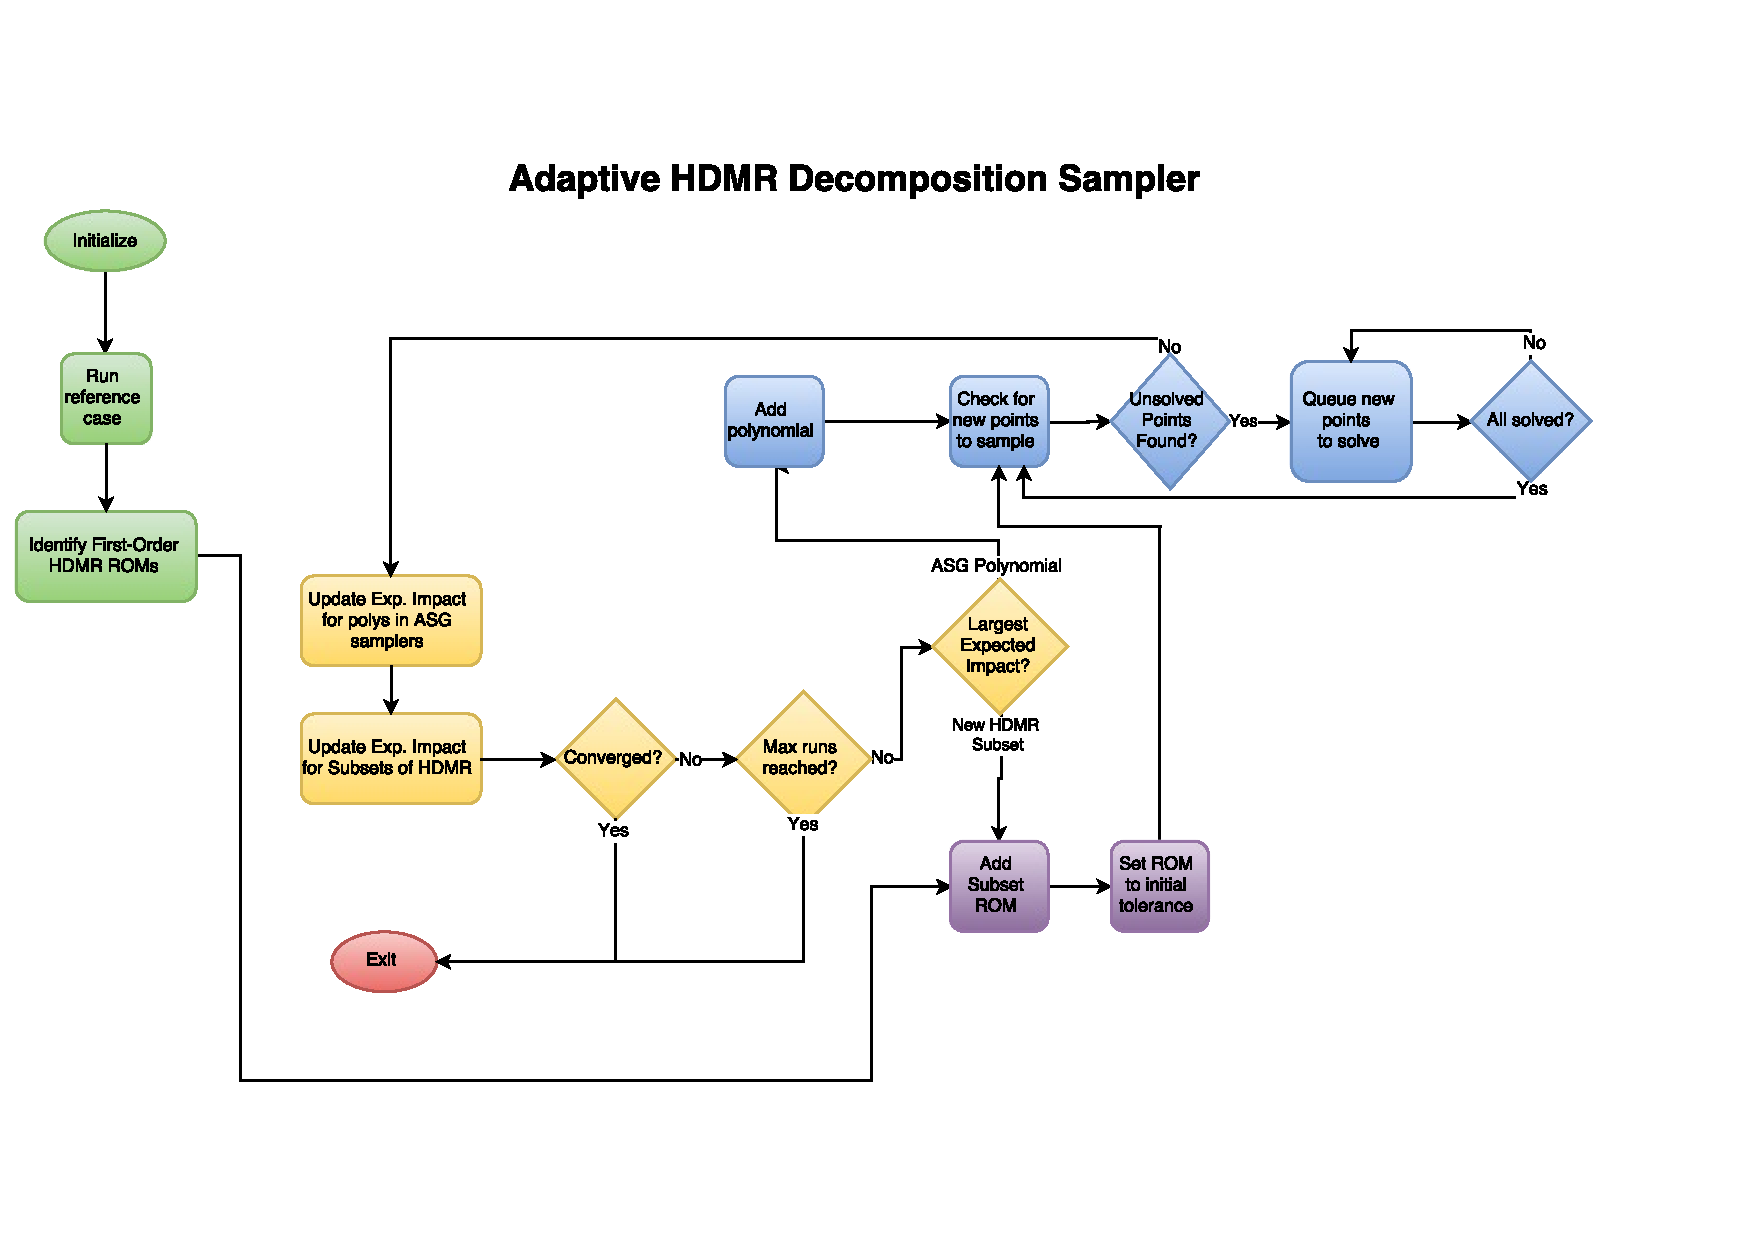
\includegraphics[width=\linewidth]{diagram-AHDMR}
  \caption{Adaptive HDMR with Adaptive Sparse Grid Flow Chart}
  \label{fig:ahdmr}
\end{figure}


Recall from section \ref{sec:adaptive sparse grid} that the impact of a polynomial within a subset generalized
polynomial chaos expansion is given by Eq. \ref{eq: poly impact},
\begin{equation}
  \tilde \eta_k = \frac{1}{N-j}\sum_{n=1}^N \eta_{k-e_n},
\end{equation}
where we omit a superscript $(y_n)$ to indicate the subset for which this polynomial is part of the generalized
polynomial chaos expansion.  As we discuss below on page~\pageref{sec: one poly per subset}, we restrict each 
polynomial to be eligible for addition to only one HDMR subset apiece, making the distinction unnecessary.  
The Sobol sensitivities provide the (current) impact of an existing subset,
\begin{equation}
  S_\beta = \frac{\text{var}\qty[h_\beta]}{\text{var}\qty[T(Y)]},
\end{equation}
computing $h$ as described in section \ref{sec:cut to anova}, and introducing subset descriptor $\beta$ which
can be any number and combination of input variables $y_n$ such that $\beta\subset Y$, or equivalently
$\beta\subset (y_1,\cdots,y_N)$.  The estimated global impact $\tilde\xi_k$ of a
polynomial $k$ within a
subset $t_\beta$ is the product of its (estimated) local and (current) subset sensitivities,
\begin{equation}
  \tilde \xi_k = \tilde\eta_k\cdot S_\beta.
\end{equation}
Analogously, the actual global impact $\xi_k$ of a polynomial $k$ within a subset $t_\beta$ is the
product of its local and subset sensitivities,
\begin{equation}
  \xi_k = \eta_k\cdot S_\beta,
\end{equation}
with $\eta_k$ given in Eq. \ref{eq: act poly impact}.
The estimated impact $\tilde S_\beta$ of adding a new subset to the HDMR expansion is the average of its
dependent subsets' Sobol sensitivities,
\begin{equation}
  \tilde S_\beta = \frac{1}{m}\hspace{-10pt} \mlsum{\gamma\subset\beta\\1+\dim(\gamma)=m}{}\hspace{-10pt} S_\gamma,
\end{equation}
where $m$ is the dimensionality of $\beta$,
\begin{equation}
  m = \dim(\beta),
\end{equation}
and by $\dim(\beta)$ we denote the dimensionality of $\beta$.  For example,
\begin{equation}
  \tilde S_{y_1,y_2} = \frac{1}{2}\qty(S_{y_1}+S_{y_2}).
\end{equation}

The philosophy behind combining polynomial impact parameters and Sobol sensitivity parameters is to provide a
means to allow the adaptive algorithm to optimize computational resources.  In effect, taking the product of
the polynomial impact with the Sobol sensitivity provides a local-to-global contribution,
\begin{equation}
  \frac{\text{local contribution}}{\text{local variance}} \cdot \frac{\text{local variance}}{\text{global
        variance}} = \frac{\text{local contribution}}{\text{global variance}}.
\end{equation}
Comparing polynomials within a subset is simple, and involves inquiring the truth of a statement like the
following:
\begin{equation}
  \tilde\eta_{k_1} \hspace{5pt}\stackrel{?}>\hspace{5pt} \tilde\eta_{k_2}.
\end{equation}
Comparing polynomials from different subsets requires only weighting them by their subset Sobol sensitivities,
\begin{equation}
  \tilde\eta_{k_1}S_{\beta_1} \hspace{5pt}\stackrel{?}>\hspace{5pt} \tilde\eta_{k_2}S_{\beta_2}.
\end{equation}
Comparing polynomials to subsets is somewhat more ambiguous,
\begin{equation}
  \tilde\eta_{k_1}S_{\beta_1} \hspace{5pt}\stackrel{?}>\hspace{5pt} \tilde S_{\beta_3}.
\end{equation}
Three cases can occur in comparing subsets to polynomials:
\begin{itemize}
  \item If $S_{\beta_1} = \tilde S_{\beta_3}$, because $\tilde\eta_{k_1}$ must be equal to or less than one,
    the algorithm will choose to add the new subset.
  \item If $S_{\beta_1} < \tilde S_{\beta_3}$, it is more reasonable to add a new subset before attempting to 
    improve the resolution of the existing subset.
  \item If $S_{\beta_1} > \tilde S_{\beta_3}$, the determination is left up to the polynomial's sensitivity.
    If the polynomial is expected to have a low impact on the Sobol sensitivity coefficient of its subset, the
    algorithm will likely choose to add a new subset.  If, however, the Sobol sensitivity coefficient is
    poorly converged, the algorithm will prefer to resolve it before trusting the estimate of the new subset's
    impact.
\end{itemize}

Because the predictive algorithm is somewhat arbitrary, we additionally offer a method to provide analysts a
tool to guide the adaptive algorithm.  By introducing a preferential factor $\alpha\in[0,2]$, the user can
push the algorithm to prefer either new subsets over polynomials or vice versa.
\begin{equation}
  \qty(\tilde\eta_{k_1})^\alpha S_{\beta_1}^{2-\alpha} \hspace{5pt}\stackrel{?}>\hspace{5pt} 
         \qty(\tilde S_{\beta_3})^{2-\alpha}.
\end{equation}
If $\alpha$ is zero, the polynomial impact is entirely ignored, and algorithm progression depends entirely on
the Sobol sensitivity data.  This means that even if a Sobol sensitivity coefficient is entirely resolves, as
long as it is the largest coefficient, additional polynomials will be added to it.  If $\alpha$ instead is 2,
the Sobol sensitivity information is ignored and only polynomial impacts are considered.  In this case, no new
subsets will ever be added.  The default algorithm is restored with $\alpha=1$.  While we recommend strongly
against $alpha=0$ and $alpha=2$, there is a range of values that can provide some manual control to either
prefer resolving polynomials ($\alpha<1$) or prefer adding new subsets ($\alpha > 1$).

The use of predictive measures to algorithmically choose a path of polynomial exploration is an addition from 
previous efforts to couple
polynomial chaos expansions with high-density model reduction.  Previously, such as in \cite{Gerstner}, the
algorithm evaluates all potential candidates then keeps the most impactful one.  While this is more guaranteed
to find the most effective path, it also is much more computationally expensive.  Even if the adaptive
algorithm guesses incorrectly, it can do so many times before matching the expense of the non-predictive
algorithm.

Whenever an iteration is taken in the algorithm, it is important to-calculate all the sensitivities and
impacts, both estimated and actual, for each subset and polynomial.  Because of the efficiencies of both the
generalized polynomial chaos expansion and high-density model reduction expansion, this is quite
computationally efficient.  Whenever a new element is added to the global expansion, it changes the total
variance, and so adjusts all the impact parameters.

When the algorithm determines a new subset should be added to the expansion, traditionally we would initialize
the subset as we would a typical adaptive sparse grid expansion, with a single first-order polynomial in each
direction making up the polynomial index set.  However, this is a poor choice for this algorithm.  Because the
subset has selected a new subset, the impact of the new subset will be zero unless it adds at least a
polynomial that is first order in all the inputs that are part of the subset.  As such, for this combined
adaptive algorithm we initialize each subset with a tensor combination of linear polynomials instead of the
traditional collection of non-interactive first-order polynomials only.

\phantomsection \label{sec: one poly per subset}
We note that the same polynomial may appear in several different subset terms and have a
different impact in each.  To simplify this problem, we restrict eligible polynomials in each subset to
include all nonzero orders for inputs on which the subset relies.  For example, the polynomial $k=(1,0,0)$ in
a three-dimensional problem is potentially eligible for subset $t_1$ but not for $t_{1,2}$.

If a subset is
selected to add a polynomial in the adaptive algorithm and the selected polynomial depends on a polynomial with 
lower effective
dimensionality, that lower-order polynomial is added to the lower-dimensional subset at the same time the
selected polynomial is added to the selected subset.  For example, consider an adaptive cut-HDMR expansion $T(x,y)$ of a
two-dimensional model $u(x,y)$ consists of three subsets $t_x$, $t_y$, and $t_{x,y}$.  Let the adaptive
polynomial set for $t_x$ be $\Lambda_x = ( (0,0),(1,0) )$, and for $t_y$ be $\Lambda_y = ( (0,0),(0,1) )$, and for
$t_{x,y}$ be $\Lambda_{x,y} =( (0,0),(0,1)(1,0),(1,1))$.  Further, let the adaptive cut-HDMR algorithm have
selected the polynomial $k=(1,2)$ to add to subset $t_{x,y}$.  Traditionally, this would require $k=(0,2)$ to
be present first.  However, because $(0,2)$ belongs to subset $t_y$, the adaptive algorithm step adds $(1,2)$
to $t_{x,y}$ and $(0,2)$ to $t_y$ simultaneously.  This is most likely to occur when there are strong
interaction effects that overshadow single-input effects.

There are several further improvements that can be made to this combined adaptive algorithm, which we discuss
in section \ref{ch:future}.
